\section{Individual Generation Process}\label{generationProcess}

If not mentioned differently, each model was trained for 10,000 iterations using a single T4 GPU in Google Colab with the High-Ram setting enabled. It is important to note that this hardware configuration does not match the specifications used in the official implementations of these models. Consequently, the results generated in this study may not be as detailed and precise. Despite these limitations, the primary purpose here is to evaluate the basic capabilities of each model, which is possible even with comparatively modest hardware standards.

To effectively demonstrate the generation process of each method, an example prompt was used: ``a robot made of plants''. The choice of this prompt was strategic as concept of a robot is inherently versatile and does not have a rigid definition in terms of appearance or composition. Furthermore, it was assumed that a simple prompt such as ``a robot'' would lead to bland models, reflecting the results observed when applying such a prompt to a 2D diffusion model, specifically Dall-E 3 \citep{dalle3}. To mitigate this, the phrase ``made out of plants'' was added. This not only countered the potential monotony of the models, but also tested the models' ability to represent intricate detail and incorporate color, particularly the various hues associated with plants. The expectation was that this addition would enrich the output of the models and provide a more comprehensive basis for evaluating their detail rendering capabilities.

\textbf{Dreamfusion}~--~The model begins by initializing an object randomly and then refines it throughout the training process. Each prompt initiates the creation of a distinct scene, meaning that even repeated usage of the same text input generates unique objects. This phenomenon is evident in the results presented in Figure~\ref{fig:generationDreamFusion}, and Figure~\ref{fig:secondRobotDreamfusion} included in the Appendix. The entire training process typically spans approximately 1.5 hours, with each iteration consuming a consistent amount of time.

\begin{figure}[ht]
    \centering
    % Subfigure for textual description
    \begin{subfigure}[b]{0.20\textwidth}
        \centering
        \fontsize{9pt}{7pt}\selectfont\text{Iteration = 100}\vspace{3cm}
        \fontsize{9pt}{7pt}\selectfont\text{Iteration = 5000}\vspace{2.85cm}
        \fontsize{9pt}{7pt}\selectfont\text{Iteration = 10000}\vspace{1.95cm}
    \end{subfigure}
    \begin{subfigure}[b]{0.20\textwidth}
        \centering
        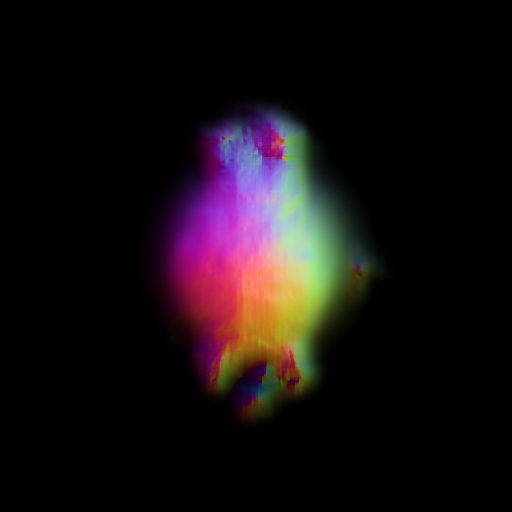
\includegraphics[width=\textwidth]{etc/a robot made out of plants/dreamfusion/dreamfusion_plantrobot_1_part2.png}
        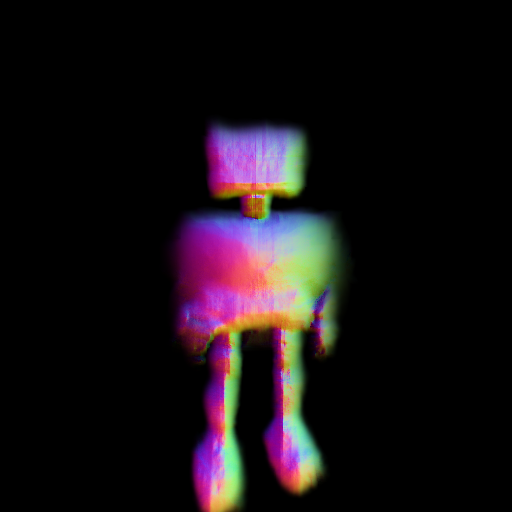
\includegraphics[width=\textwidth]{etc/a robot made out of plants/dreamfusion/dreamfusion_plantrobot_5000_part2.png}
        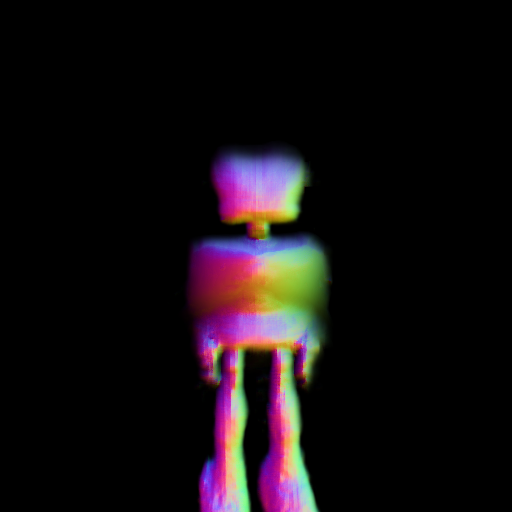
\includegraphics[width=\textwidth]{etc/a robot made out of plants/dreamfusion/dreamfusion_plantrobot_10000_part2.png}
        \caption{}
    \end{subfigure}
    \begin{subfigure}[b]{0.20\textwidth}
        \centering
        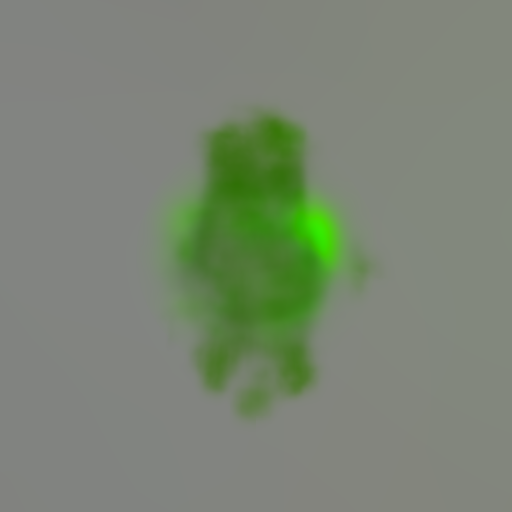
\includegraphics[width=\textwidth]{etc/a robot made out of plants/dreamfusion/dreamfusion_plantrobot_1_part1.png}
        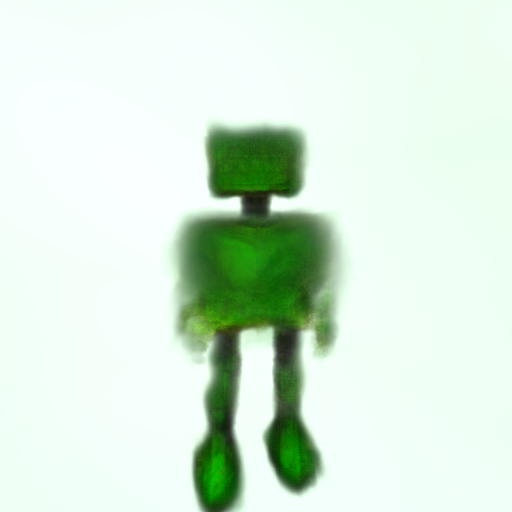
\includegraphics[width=\textwidth]{etc/a robot made out of plants/dreamfusion/dreamfusion_plantrobot_5000_part1.png}
        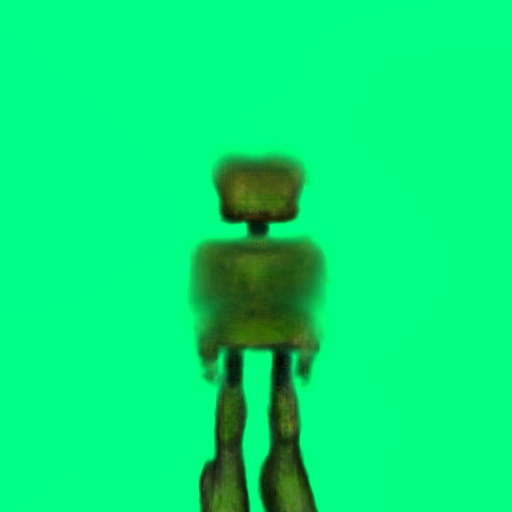
\includegraphics[width=\textwidth]{etc/a robot made out of plants/dreamfusion/dreamfusion_plantrobot_10000_part1.png}
        \caption{}
    \end{subfigure}
    % Subfigure 3
    \hspace{.5cm}
    \begin{subfigure}[b]{0.252\textwidth}
        \centering
        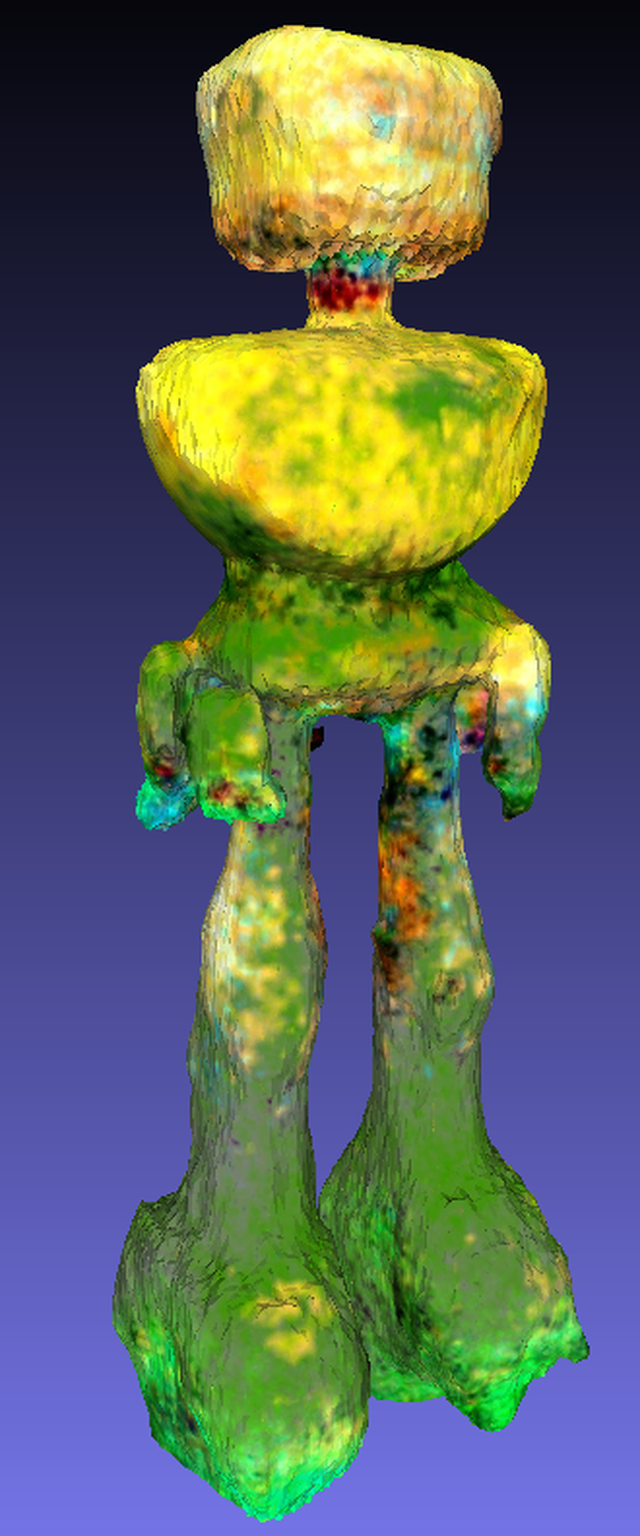
\includegraphics[width=\textwidth]{etc/a robot made out of plants/dreamfusion/dreamfusion_plantrobot_model_resized.png}
        \caption{}
    \end{subfigure}
    \caption{The generation process of Dreamfusion using the prompt ``a robot made out of plants''. Section (c) shows a snapshot of the final mesh generated.}~\label{fig:generationDreamFusion}
\end{figure}

As can be seen in Figure~\ref{fig:generationDreamFusion} parts a and b, the object and its texture are generated simultaneously. The process starts with a small dot that gradually transforms into a more complex shape. At the 100th iteration, the original dot begins to transform into a recognizable shape, and a green hue resembling plant coloration is created. At the 5000th iteration, distinct features such as two legs, a square body and a square head become visible, all retaining the same shade of green. At the last, 10,000th iteration, the model shows a background and small arms sticking out of the robot's body.
Part c of the figure showcases the rendered mesh opened in Meshlab \citep{meshLab}, highlighting alterations made by Threestudio, such as duplicate removal and hole filling. These modifications account for the slight differences between the final mesh and the validation images produced during training. Interestingly, the final mesh lacks detailed plant-like features, one could only assume that the legs kind of resemble moss, but this remains speculation. The mesh primarily shows basic shapes, including a square head, a torso with small protruding rods that could be arms, and large legs. Remarkably, the upper half of the body in the final mesh takes on a yellowish color that differs from the green of the earlier validation images. The reason for this color change remains unclear.

\textbf{Fantasia3D}~--~Generating 3D models can be initialised in multiple ways. The first is to just use the prompt. For this approach, Fantasia3D automatically uses a perfect sphere to initialise its mesh and begins its trainig from there. The second approach is to initially already specify this spheres initial values \([0.5, 0.5, 0.5]\) with differnet ones which would roughly describe the desired object by modifying its values according to \([depth, width, height]\). The last approach would be to initialise the mesh with a custom .obj that already acts as a rough shape input.~\ref{fig:generationFantasia} shows its approach for using nothing but the prompt for generating the plant Robot. 

\begin{figure}[ht]
    \centering
    % Subfigure for textual description
    \begin{subfigure}[b]{0.20\textwidth}
        \centering
        \fontsize{9pt}{7pt}\selectfont\text{Iteration = 0}\vspace{3cm}
        \fontsize{9pt}{7pt}\selectfont\text{Iteration = 5000}\vspace{2.85cm}
        \fontsize{9pt}{7pt}\selectfont\text{Iteration = 10000}\vspace{1.95cm}
    \end{subfigure}
    \begin{subfigure}[b]{0.20\textwidth}
        \centering
        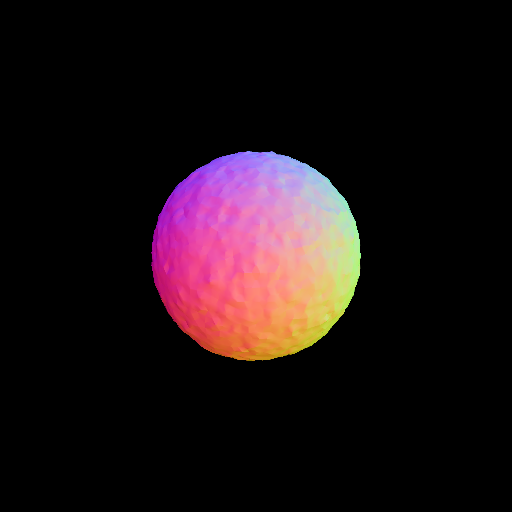
\includegraphics[width=\textwidth]{etc/a robot made out of plants/fantasia3d/fantasia_coarse_robot_0_part2.png}
        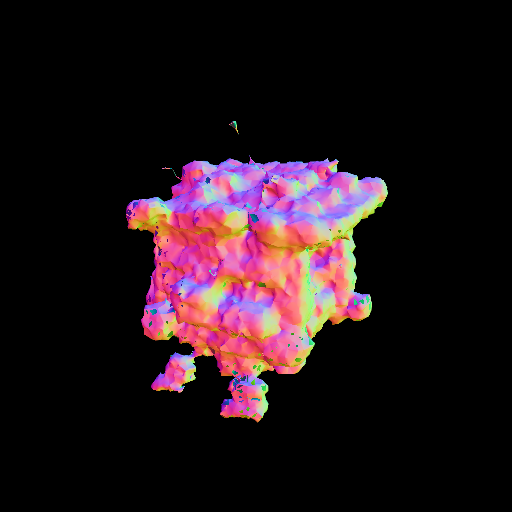
\includegraphics[width=\textwidth]{etc/a robot made out of plants/fantasia3d/fantasia_coarse_robot_5000_part2.png}
        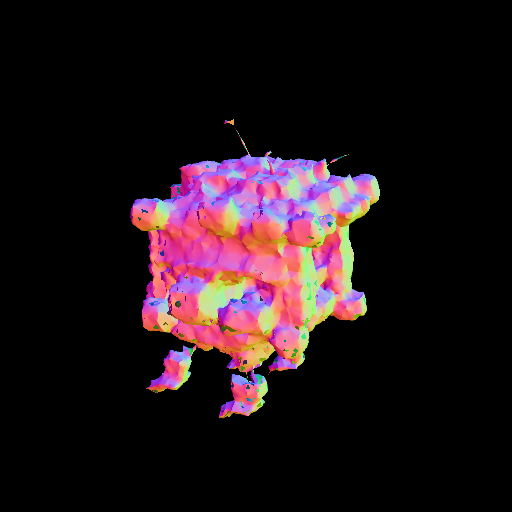
\includegraphics[width=\textwidth]{etc/a robot made out of plants/fantasia3d/fantasia_coarse_robot_10000_part2.png}
        \caption{}
    \end{subfigure}
    \begin{subfigure}[b]{0.20\textwidth}
        \centering
        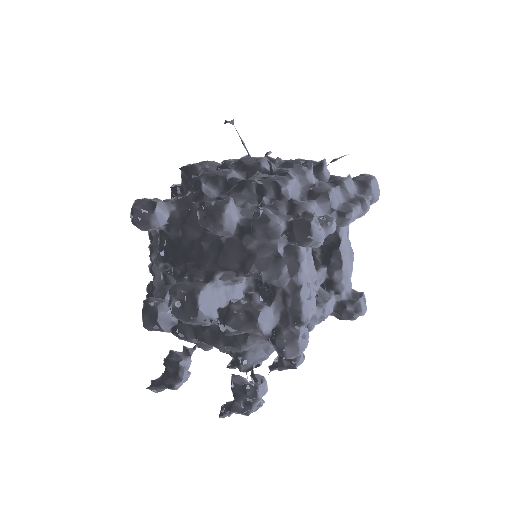
\includegraphics[width=\textwidth]{etc/a robot made out of plants/fantasia3d/fantasia_refine_robot_0_part1.png}
        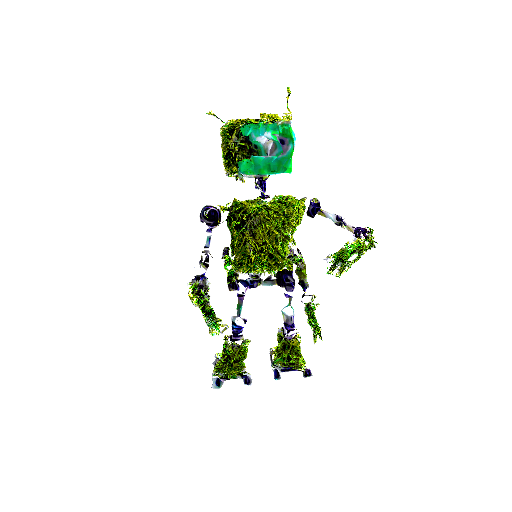
\includegraphics[width=\textwidth]{etc/a robot made out of plants/fantasia3d/fantasia_refine_robot_5000_part1.png}
        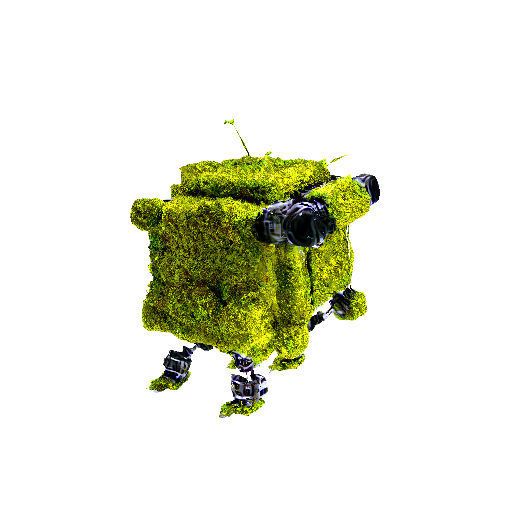
\includegraphics[width=\textwidth]{etc/a robot made out of plants/fantasia3d/fantasia_refine_robot_10000_part1.png}
        \caption{}
    \end{subfigure}
    % Subfigure 3
    \begin{subfigure}[b]{0.37\textwidth}
        \centering
        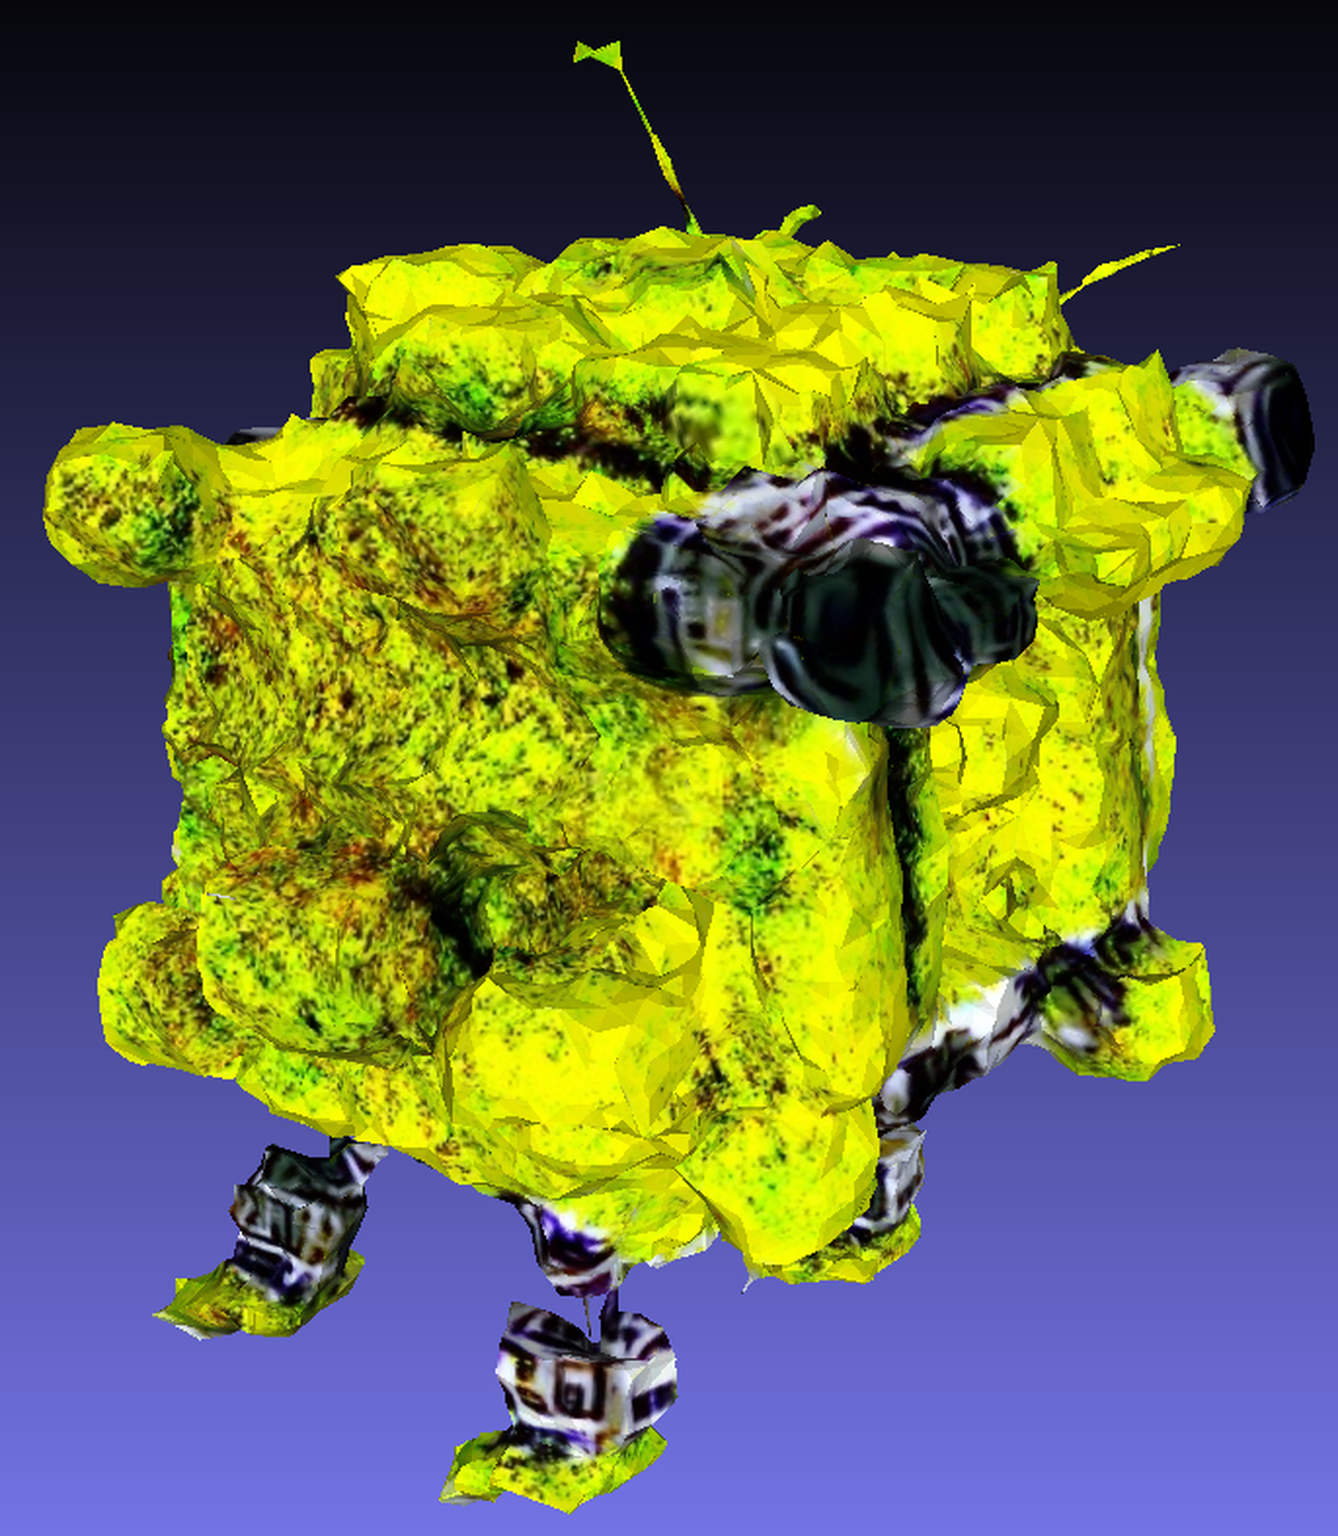
\includegraphics[width=\textwidth]{etc/a robot made out of plants/fantasia3d/fantasia_plantrobot_model_resized.png}
        \caption{}
    \end{subfigure}
    \caption{a: Fantasia3D starting with only a perfect square and refining this according to the prompt ``a robot made out of plants''. In b: only the appearance of the model gets refined. Image c shows the rendered model }~\label{fig:generationFantasia}
\end{figure}


\begin{figure}[ht]
    \centering
      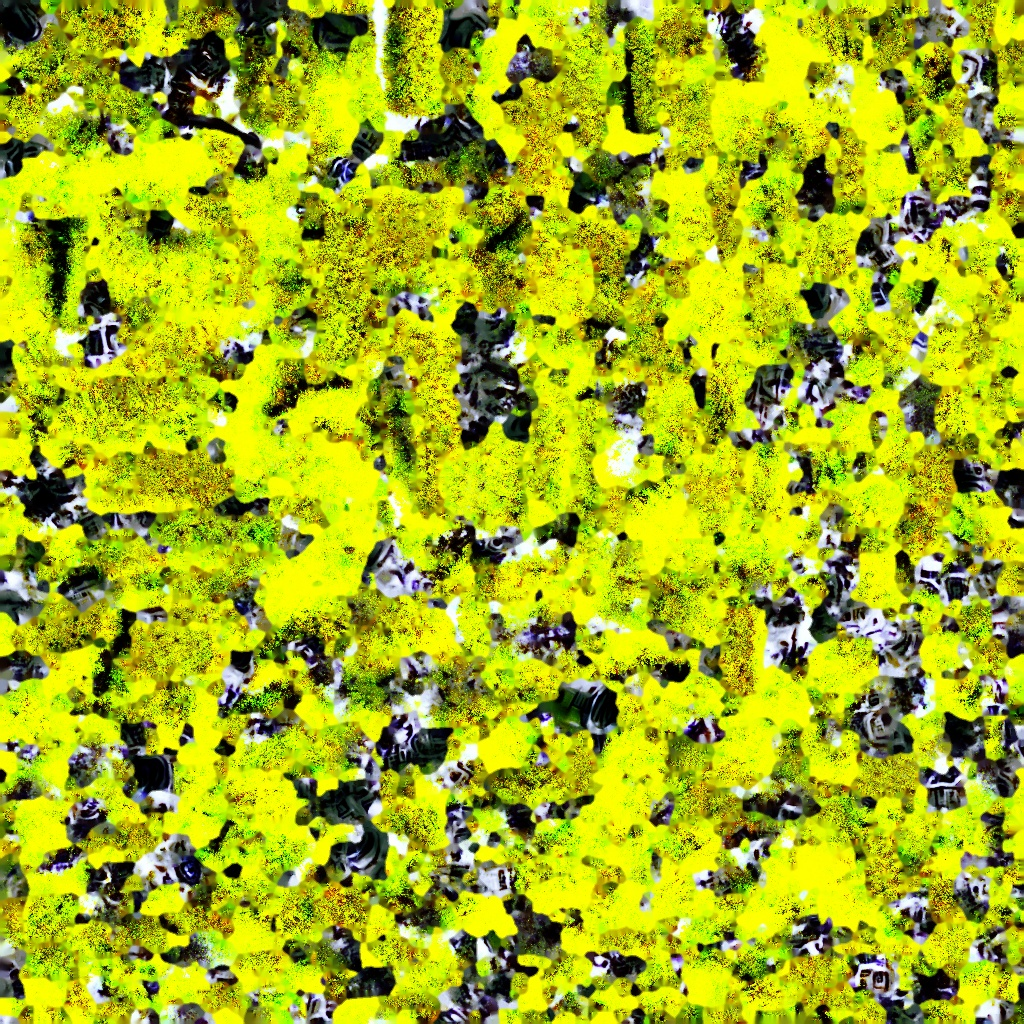
\includegraphics[width=.2\columnwidth]{etc/a robot made out of plants/fantasia3d/fantasia_refine_robot_kd}
      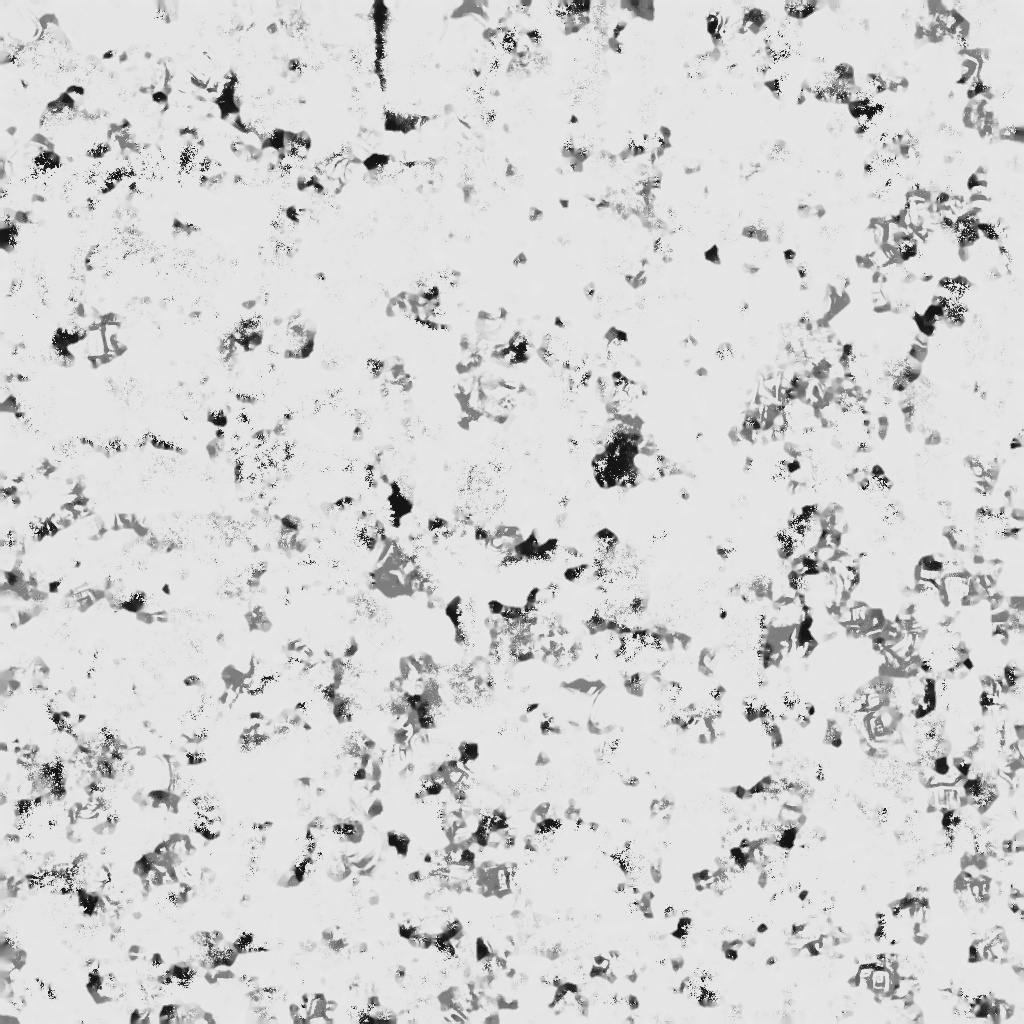
\includegraphics[width=.2\columnwidth]{etc/a robot made out of plants/fantasia3d/fantasia_refine_robot_roughness}
      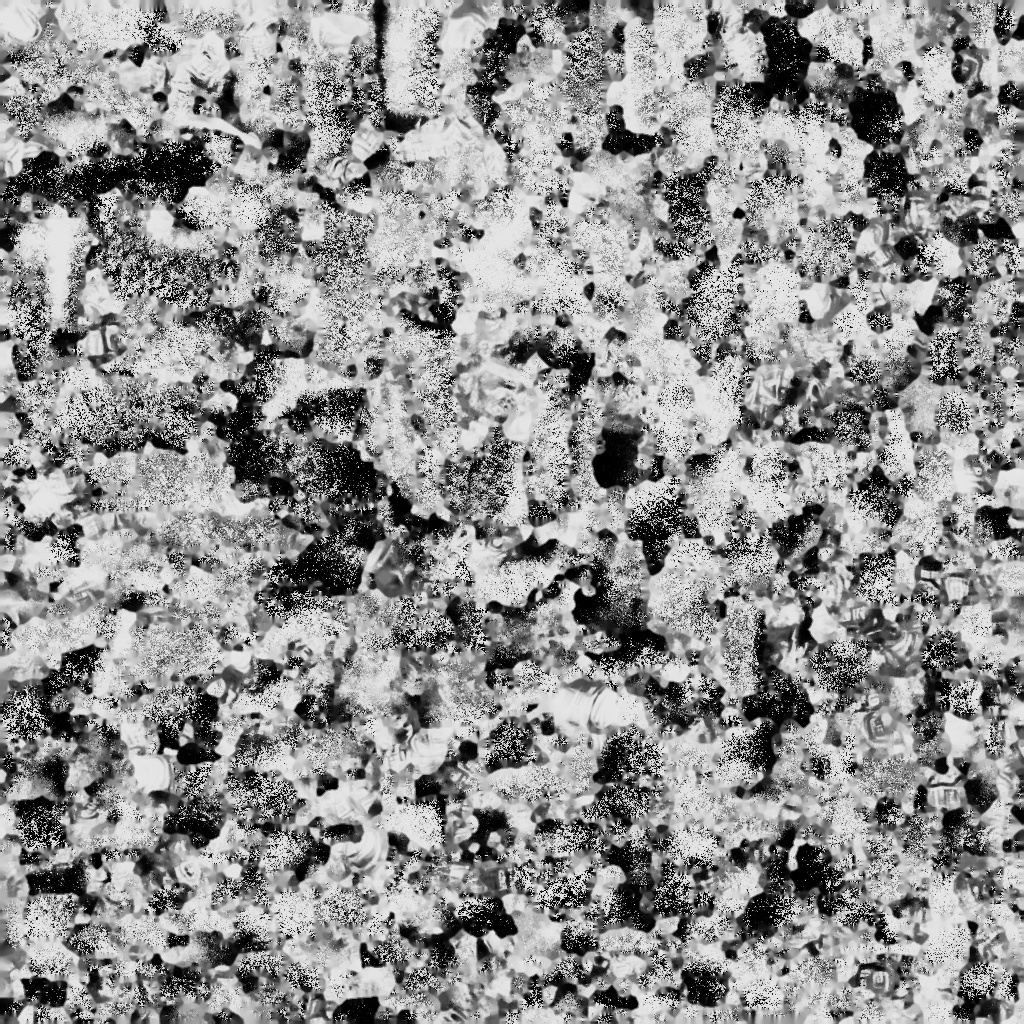
\includegraphics[width=.2\columnwidth]{etc/a robot made out of plants/fantasia3d/fantasia_refine_robot_metallic}
      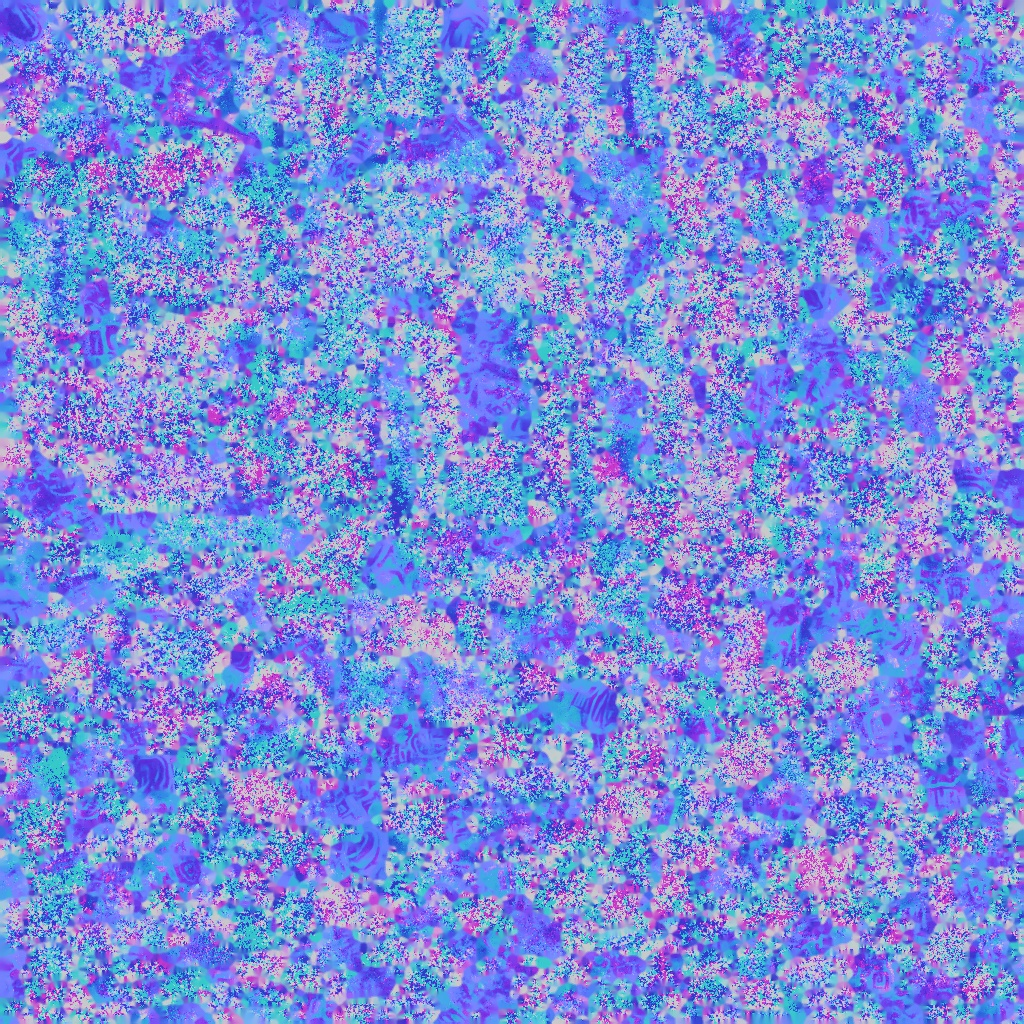
\includegraphics[width=.2\columnwidth]{etc/a robot made out of plants/fantasia3d/fantasia_refine_robot_normal}
      \caption{generated textures from Fantasia3D}~\label{fig:texturesFantasia}
  \end{figure}

\textbf{Magic3D}~--~Test 

\textbf{magic123}~--~Test

\textbf{Wonder3D}~--~Test